\documentclass[12pt,a4paper]{article}

% ===== Codificación y español =====
\usepackage[utf8]{inputenc}
\usepackage[T1]{fontenc}
\usepackage[spanish, es-tabla]{babel}

% ===== Márgenes y gráficos =====
\usepackage{geometry}
\geometry{margin=2.5cm}
\usepackage{graphicx}
\usepackage{float}        % [H] para fijar figuras/tablas
\usepackage{subcaption}   % subfiguras
\usepackage{booktabs}     % tablas más bonitas
\usepackage{amsmath}

% ===== Hipervínculos y referencias =====
\usepackage{hyperref}
\hypersetup{
  colorlinks=true,
  linkcolor=black,
  citecolor=black,
  urlcolor=blue
}

\usepackage{siunitx}
\sisetup{
  output-decimal-marker = {.}, % decimal con punto
  group-separator = {,},       % miles con coma
  group-minimum-digits = 4,
  group-digits = integer,
  table-number-alignment = center,
  round-mode = places,
  detect-all = true            % ignora configuraciones de babel
}

% Ayuda al manejo de tablas
\usepackage{tabularx}
\usepackage{adjustbox}
\usepackage{longtable}

% cleveref mejora \ref: escribe "Figura 1", "Tabla 2", etc.
\usepackage[capitalise,noabbrev]{cleveref}

% Ajuste de nombres en cleveref
\crefname{figure}{figura}{figuras}
\Crefname{figure}{Figura}{Figuras}
\crefname{subfigure}{subfigura}{subfiguras}
\Crefname{subfigure}{Subfigura}{Subfiguras}
\crefname{table}{tabla}{tablas}
\Crefname{table}{Tabla}{Tablas}
\crefname{equation}{ecuación}{ecuaciones}
\Crefname{equation}{Ecuación}{Ecuaciones}
\crefname{section}{sección}{secciones}
\Crefname{section}{Sección}{Secciones}

% Listas más controlables
\usepackage{enumitem}

\graphicspath{{figuras/}}

% ===== Título y autoría =====
\title{\textbf{Agrupamiento jerarquico}}
\author{Haessler Joan Ortiz Moncada \\[0.5cm]
        Universidad Distrital Francisco José de Caldas \\
        Facultad de Ingeniería \\
        Curso: Big Data}
\date{\today}

\begin{document}

\maketitle

\section{Introducción}
Este documento presenta el desarrollo de los ejercicios planteados en el \texttt{Taller\_6} 
del curso de Big Data , documentando los hallazgos y análisis correspondientes. Este taller se 
centra principalmente en el abordaje de dos \textit{\textit{datasets}}: uno proporcionado por el profesor de la clase, 
denominado \texttt{data\_clusters.mat}, y otro descargado de \href{http://archive.ics.uci.edu/dataset/406/anuran+calls+mfccs}{Anuran Calls}. 
A partir de estos conjuntos de datos se busca implementar y practicar metodologías de clasificación no supervisada, específicamente 
agrupamiento jerarquico.

\section{Metodología}
En cuanto al orden, el trabajo se desarrolla conforme a lo establecido en el \texttt{Taller\_6}. 
Respecto a la forma, la implementación de los modelos, la preparación de los datos y la visualización de 
los resultados se llevan a cabo mediante un archivo de \texttt{Jupyter Notebook} desarrollado en Colab. 
Cabe aclarar que la Inteligencia Artificial (IA) Gemini asistió en la generación del código requerido. 
Por último, el código producido, los datos implementados y el informe generado, pueden consultarse en la 
carpeta \texttt{taller\_6} del repositorio \href{https://github.com/HaesslerOrtiz/bigdata}{bigdata\_repositorio} 
de GitHub.

\section{Desarrollo}
El \texttt{Taller\_6} consta de dos ítems principales: el primero requiere implementar el método de agrupamiento jerárquico 
en el dataset \texttt{data\_clusters.mat} para definir el número óptimo de \textit{clusters}, lo cual debe complementarse con la 
implementación de dendrogramas y la evaluación del rendimiento del modelo mediante el índice de \textit{Silhouette} 
y el análisis de la Suma de Errores Cuadráticos (\texttt{SSE}, por sus siglas en inglés); mientras que el segundo ítem también requiere 
la aplicación del agrupamiento jerárquico para entrenar un modelo con el dataset \texttt{Anuran Calls}, una base de datos multiclase de 
sonidos de ranas, donde el objetivo es agrupar (enfoque no supervisado) o clasificar (enfoque semi-supervisado), según 
corresponda, las características \texttt{familia} y \texttt{género}.

\subsection{Agrupamiento jerarquico con data\_clusters.mat}
Teniendo el dataset \texttt{data\_clusters.mat}, se etiquetan sus dos columnas o características como \texttt{A} y \texttt{B}; 
se verifica que su tamaño es \(135 \times 2\), que ambas variables son de tipo \texttt{float} y que el conjunto no presenta valores nulos. 
Con el fin de facilitar su manipulación en el contexto de \texttt{Python}, se decide transformarlo a un archivo \texttt{.csv}. Como métodos para 
generar los dendrogramas se decidió emplear tres esquemas de enlace: enlace simple, enlace de centroide y enlace completo. Estos permiten 
contrastar cómo varía la estructura jerárquica según el criterio de agrupación (distancia mínima entre pares, distancia al centroide y 
distancia máxima entre pares, respectivamente) y se ilustran en la \Cref{fig:dendrogramas}. La distancia entre puntos se calcula mediante la 
métrica euclidiana.

\begin{figure}[H]
    \centering
    \begin{subfigure}{0.32\textwidth}
        \centering
        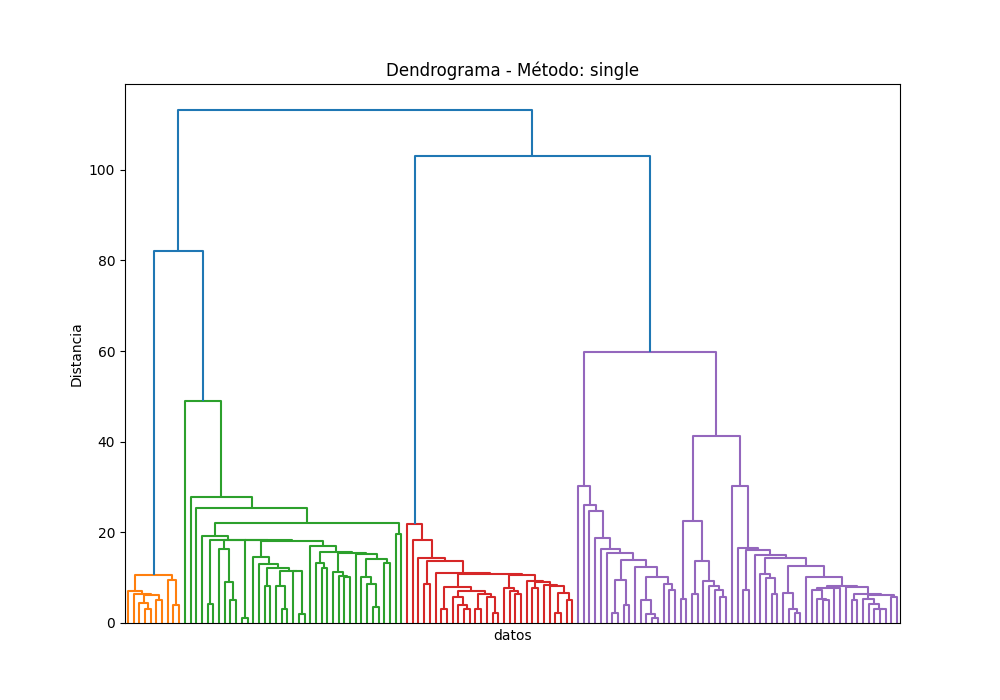
\includegraphics[width=\textwidth]{dendrograma_single.png}
        \caption{Enlace simple}
        \label{fig:dendrograma_enlace_simple}
    \end{subfigure}
    \hfill
    \begin{subfigure}{0.32\textwidth}
        \centering
        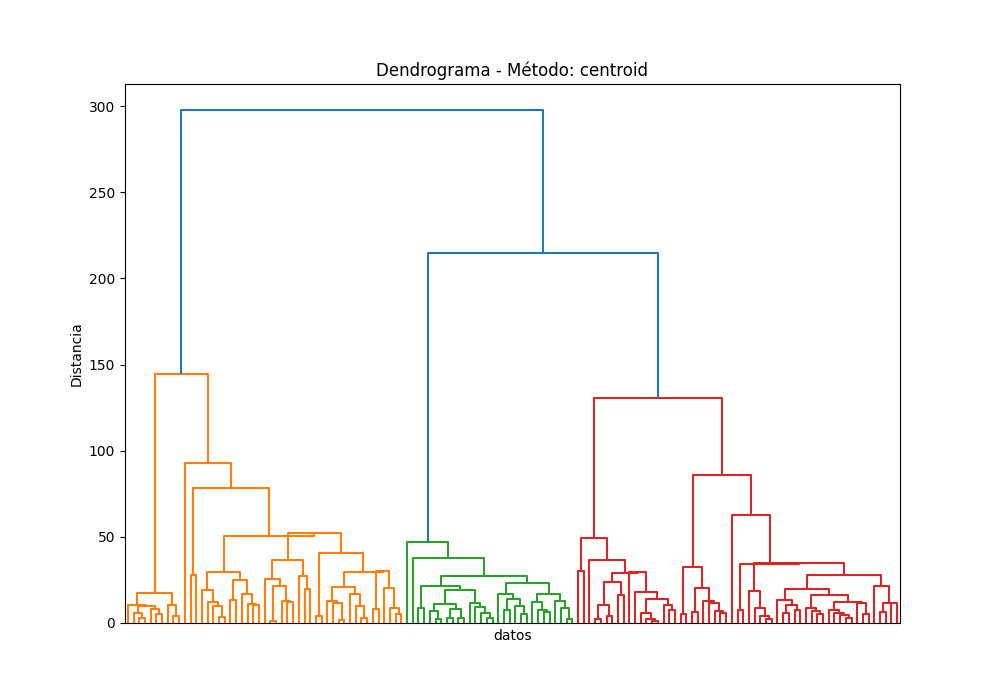
\includegraphics[width=\textwidth]{dendrograma_centroid.png}
        \caption{Enlace de centroide}
        \label{fig:dendrograma_enlace_centroide}
    \end{subfigure}
    \hfill
    \begin{subfigure}{0.32\textwidth}
        \centering
        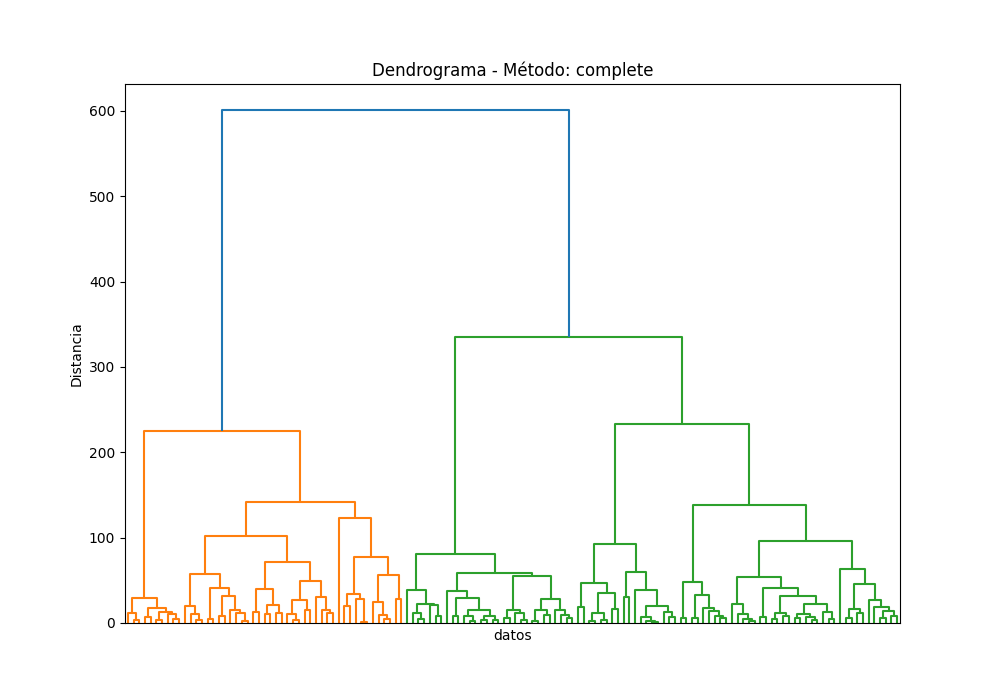
\includegraphics[width=\textwidth]{dendrograma_complete.png}
        \caption{Enlace completo}
        \label{fig:dendrograma_enlace_completo}
    \end{subfigure}
    \caption{Dendrogramas con diferentes métodos de enlace.}
    \label{fig:dendrogramas}
\end{figure}

En los tres dendrogramas se notan comportamientos distintos: con \emph{enlace simple} los datos se van “pegando” de a 
poquitos y forman cadenas largas, por lo que la separación entre grupos no queda muy clara; con \emph{enlace centroide} 
los grupos aparecen más equilibrados y es fácil imaginar tres conjuntos principales; con \emph{enlace completo} la 
separación es la más nítida, porque prioriza que cada grupo quede bien compacto y distinto de los demás. En 
resumen, para este conjunto de datos conviene \texttt{a priori} quedarse con \emph{enlace completo} y, como alternativa 
cercana, \emph{centroide}; en ambos casos un corte natural del árbol sugiere trabajar con dos o tres grupos.

Como forma de cuantificar la calidad del agrupamiento, se decide calcular el índice de \textit{Silhouette} y la 
\texttt{SSE} para cada método de enlace, variando el número de \textit{clusters} entre 2 y 10. Realmente no se tiene un 
criterio estricto del porqué se define ese rango, pero se asume que es un intervalo razonable para este conjunto de datos. Tanto 
para \textit{Silhouette} y \texttt{SSE} se implementaron estrategias para detener su cálculo en caso de que empeorara el 
rendimiento del coeficiente y el segundo entrara en una meseta, respectivamente. Para esta labor si se implementó una estandarización 
previa de los datos. Los resultados se presentan en las \Cref{fig:silhouette_sse_single,fig:silhouette_sse_centroid,fig:silhouette_sse_complete}.

\begin{figure}[H]
  \centering
  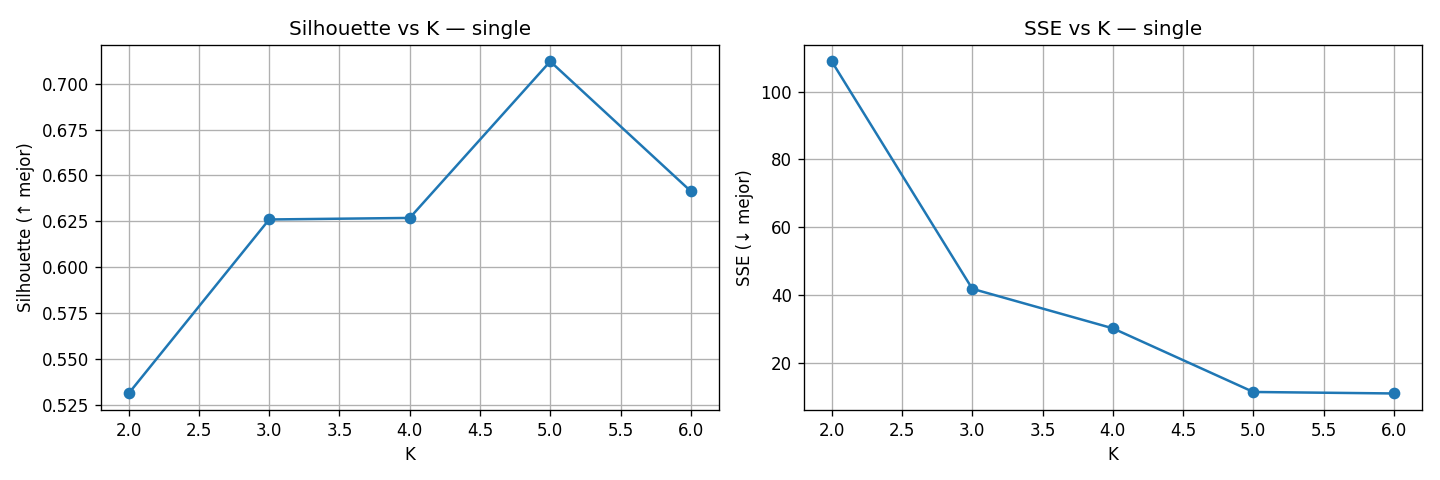
\includegraphics[width=\textwidth]{jerarquico_single_sil_sse.png}
  \caption{Silhouette y SSE para enlace simple.}
  \label{fig:silhouette_sse_single}
\end{figure}

\begin{figure}[H]
  \centering
  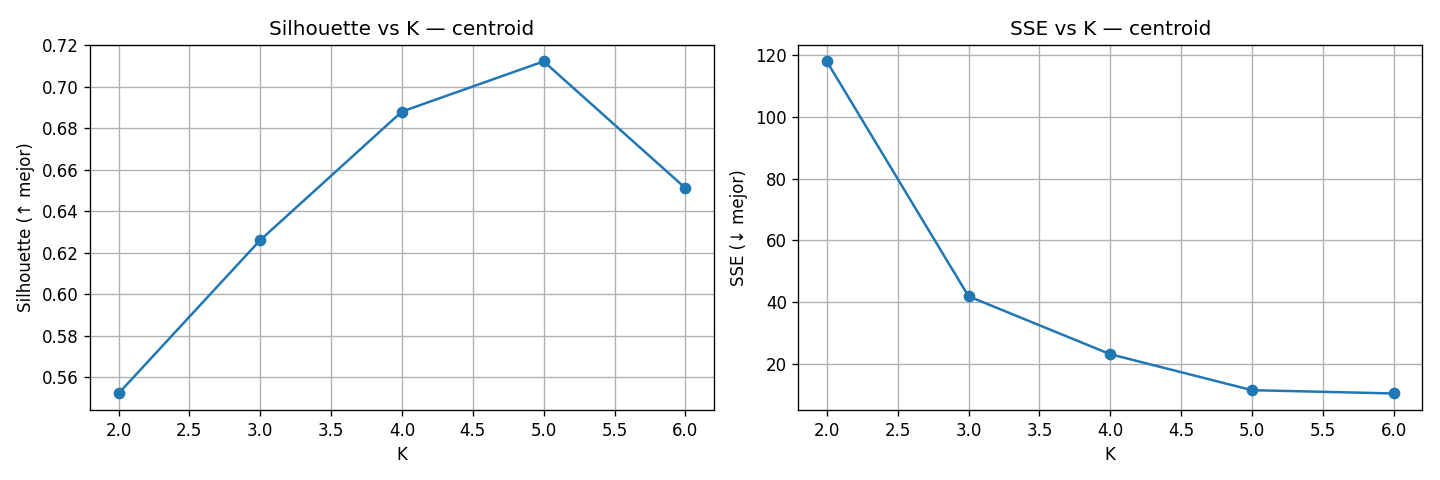
\includegraphics[width=\textwidth]{jerarquico_centroid_sil_sse.png}
  \caption{Silhouette y SSE para enlace de centroide.}
  \label{fig:silhouette_sse_centroid}
\end{figure}

\begin{figure}[H]
  \centering
  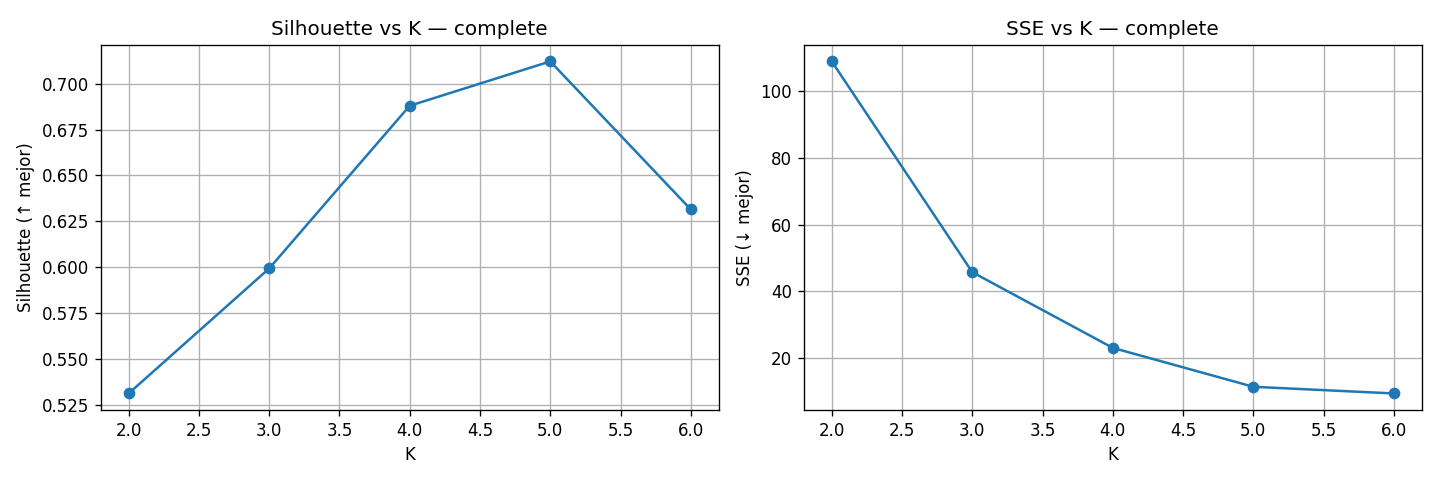
\includegraphics[width=\textwidth]{jerarquico_complete_sil_sse.png}
  \caption{Silhouette y SSE para enlace completo.}
  \label{fig:silhouette_sse_complete}
\end{figure}

A partir de los gráficos recién mostrados, se observa que los tres métodos (enlace simple, enlace de centroide y enlace completo) 
producen resultados prácticamente indistinguibles: en todos los casos, la mejor elección para la cantidad de grupos es \(k=5\). Esto 
sugiere que, para el conjunto de datos evaluado, no hay una ventaja apreciable en preferir uno u otro criterio de enlace.

\noindent\textbf{Nota}: el \texttt{Taller\_6} requería que a partir de los dendogramas se compararan las agrupaciones que generó cada 
tipo de enlace, y que a partir de ello se realizará un histograma que permitiera evaluar aquellas agrupaciones comunes, sin embargo, 
resulta complejo visualizar esta tarea. Tal vez una propuesta similar, sería la de evaluar cuántas veces un par de datos queda en el 
mismo clúster, sin llegar a identificar cuáles son los datos que se están agrupando.

\subsection{Agrupamiento jerarquico con Anuran Calls}
El segundo ítem de \texttt{Taller\_6} utiliza el conjunto de datos \texttt{Anuran Calls}, que contiene grabaciones de llamadas de 
ranas y características acústicas extraídas. El objetivo es agrupar las observaciones según \texttt{familia} y \texttt{género}. Para 
el análisis no supervisado se emplean únicamente las características numéricas, descartando las variables categóricas y la última 
característica numérica, ya que solo identifica la grabación y no aporta información al agrupamiento. En el enfoque supervisado se 
genera una etiqueta compuesta que combina \texttt{familia} y \texttt{género}, de modo que cada combinación única constituye una clase. Durante 
la preparación de los datos se verifica la ausencia de valores nulos y no se aplica estandarización, puesto que todas las características 
numéricas están en la misma escala (entre $-1$ y $1$). El conjunto de datos original tiene un tamaño de \(7195 \times 22\) y no posee 
valores nulos. 

\subsubsection{Análisis No supervisado}
Para el análisis no supervisado, se eligió la técnica \texttt{$k$-medoids} para la identificación de protogrupos, con la intención de no 
realizar el agrupamiento jerárquico directamente sobre el conjunto de datos completo, dada su considerable dimensión, con esto se reduce 
el tiempo y complejidad del computo. Se probó con distintos tamaños (g) para definir los protogrupos, eligiendo finalmente \(g=80\) como el 
valor con mejor rendimiento según el índice de \textit{Silhouette}. Este tamaño es la cantidad de protogrupos que se utilizarán como entrada para el 
agrupamiento jerárquico. Para los tamaños de los protogrupos se evaluaron los valores \(g = \{80, 100, 120, 150\}\), como regla deben ser de un tamaño 
mucho mayor al que probablemente se elija para \(k\) en el agrupamiento jerárquico. La \Cref{fig:silhouette_vs_g_kmedoids} muestra el desempeño del índice 
de \textit{Silhouette} para diferentes valores de \(g\).

\begin{figure}[H]
  \centering
  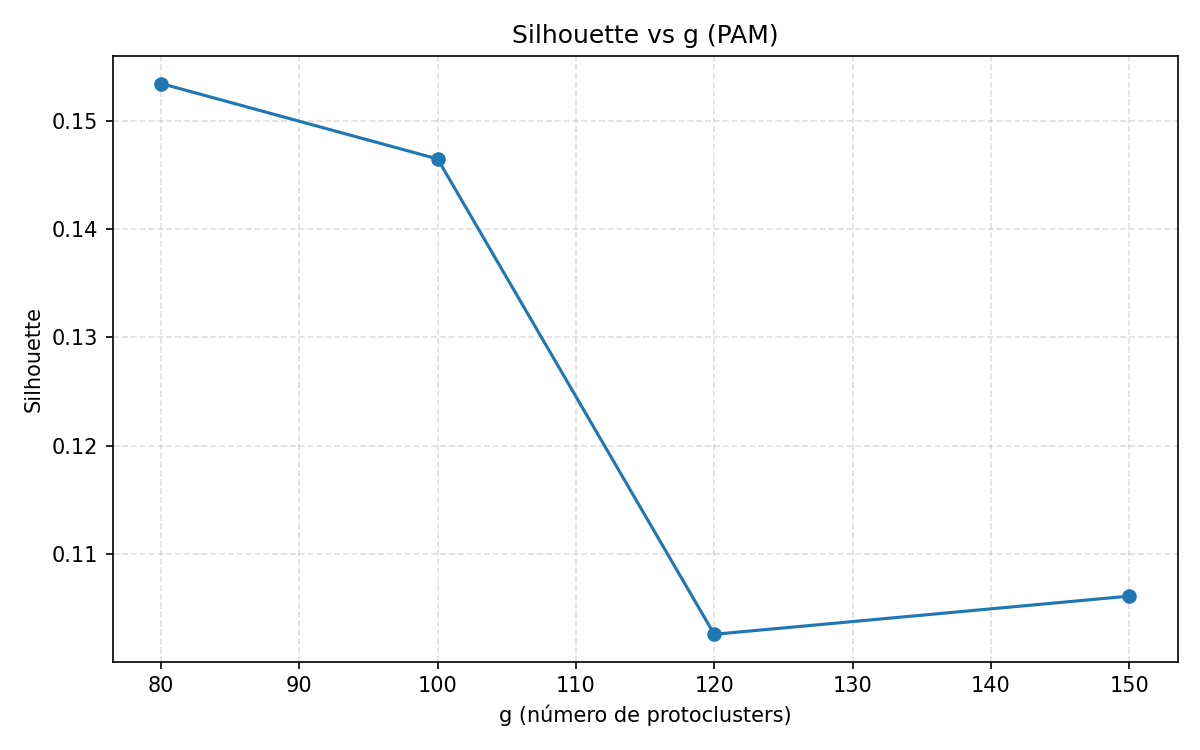
\includegraphics[width=0.7\textwidth]{silhouette_vs_g_kmedoids.png}
  \caption{Silhouette para diferentes tamaños de protogrupos \(g\).}
  \label{fig:silhouette_vs_g_kmedoids}
\end{figure}

Posteriormente, se aplicaron los métodos de (\textit{single linkage}) y (\textit{complete linkage}) para generar los respectivos dendrogramas. La 
\Cref{fig:dendrogramas_anuran} muestra los dendrogramas generados.

\begin{figure}[H]
    \centering
    \begin{subfigure}{0.45\textwidth}
        \centering
        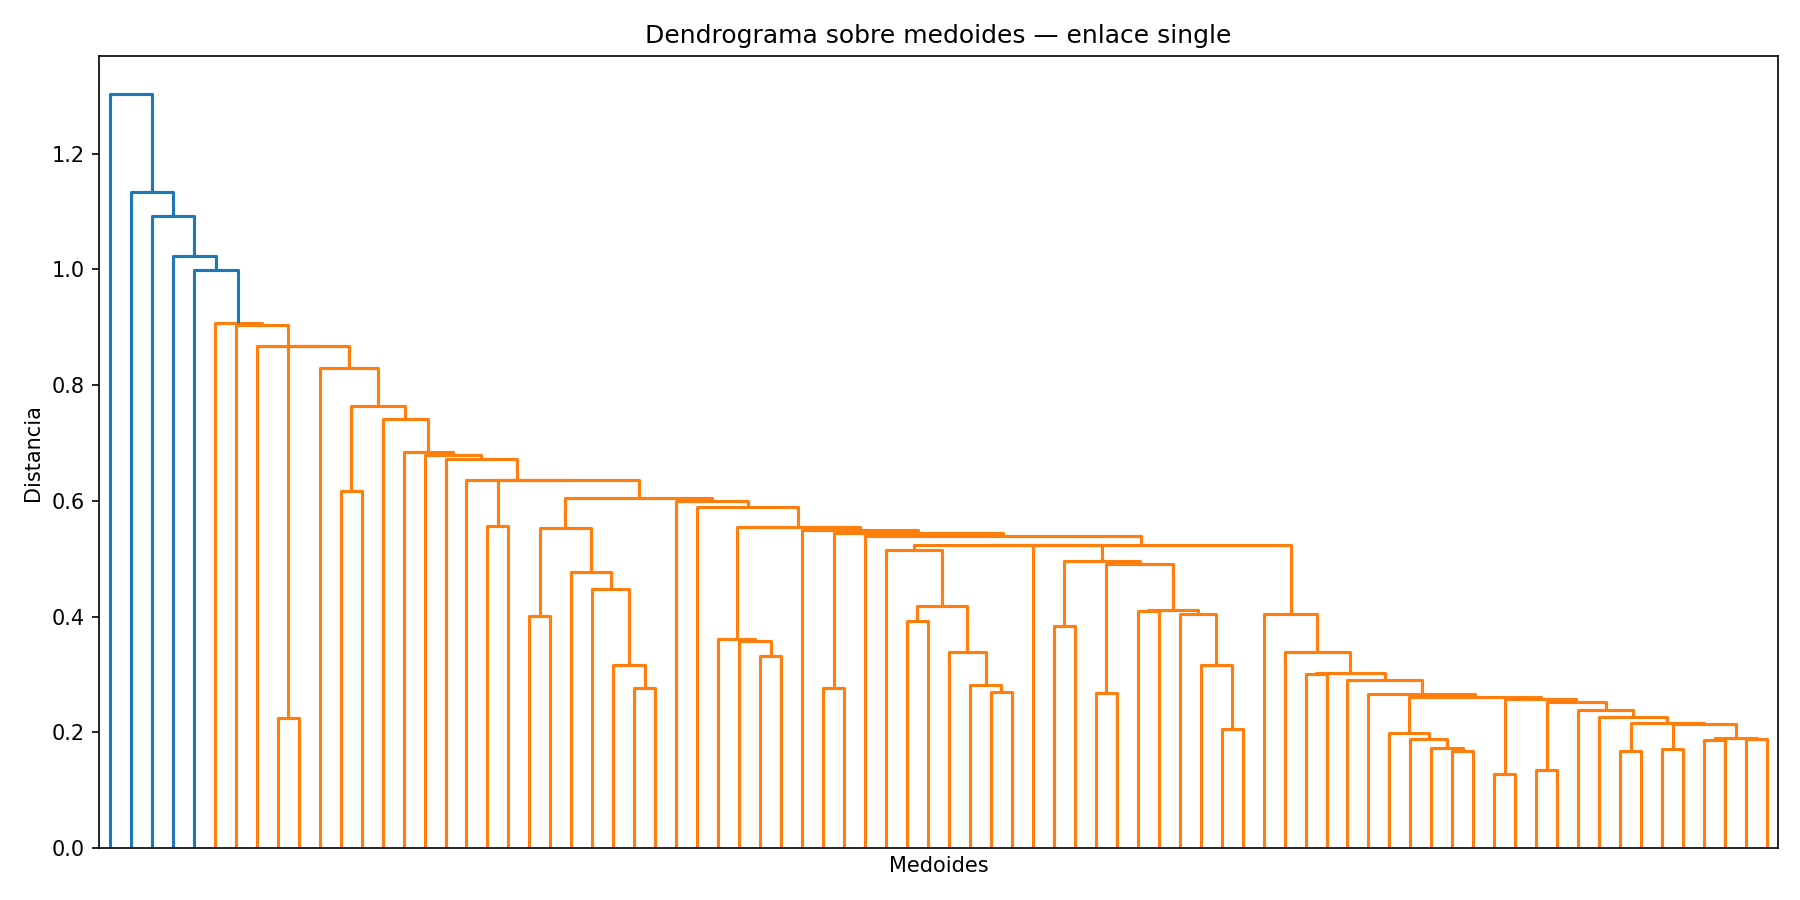
\includegraphics[width=\textwidth]{dendrograma_medoides_single.png}
        \caption{Enlace simple}
        \label{fig:dendrograma_anuran_single}
    \end{subfigure}
    \hfill
    \begin{subfigure}{0.45\textwidth}
        \centering
        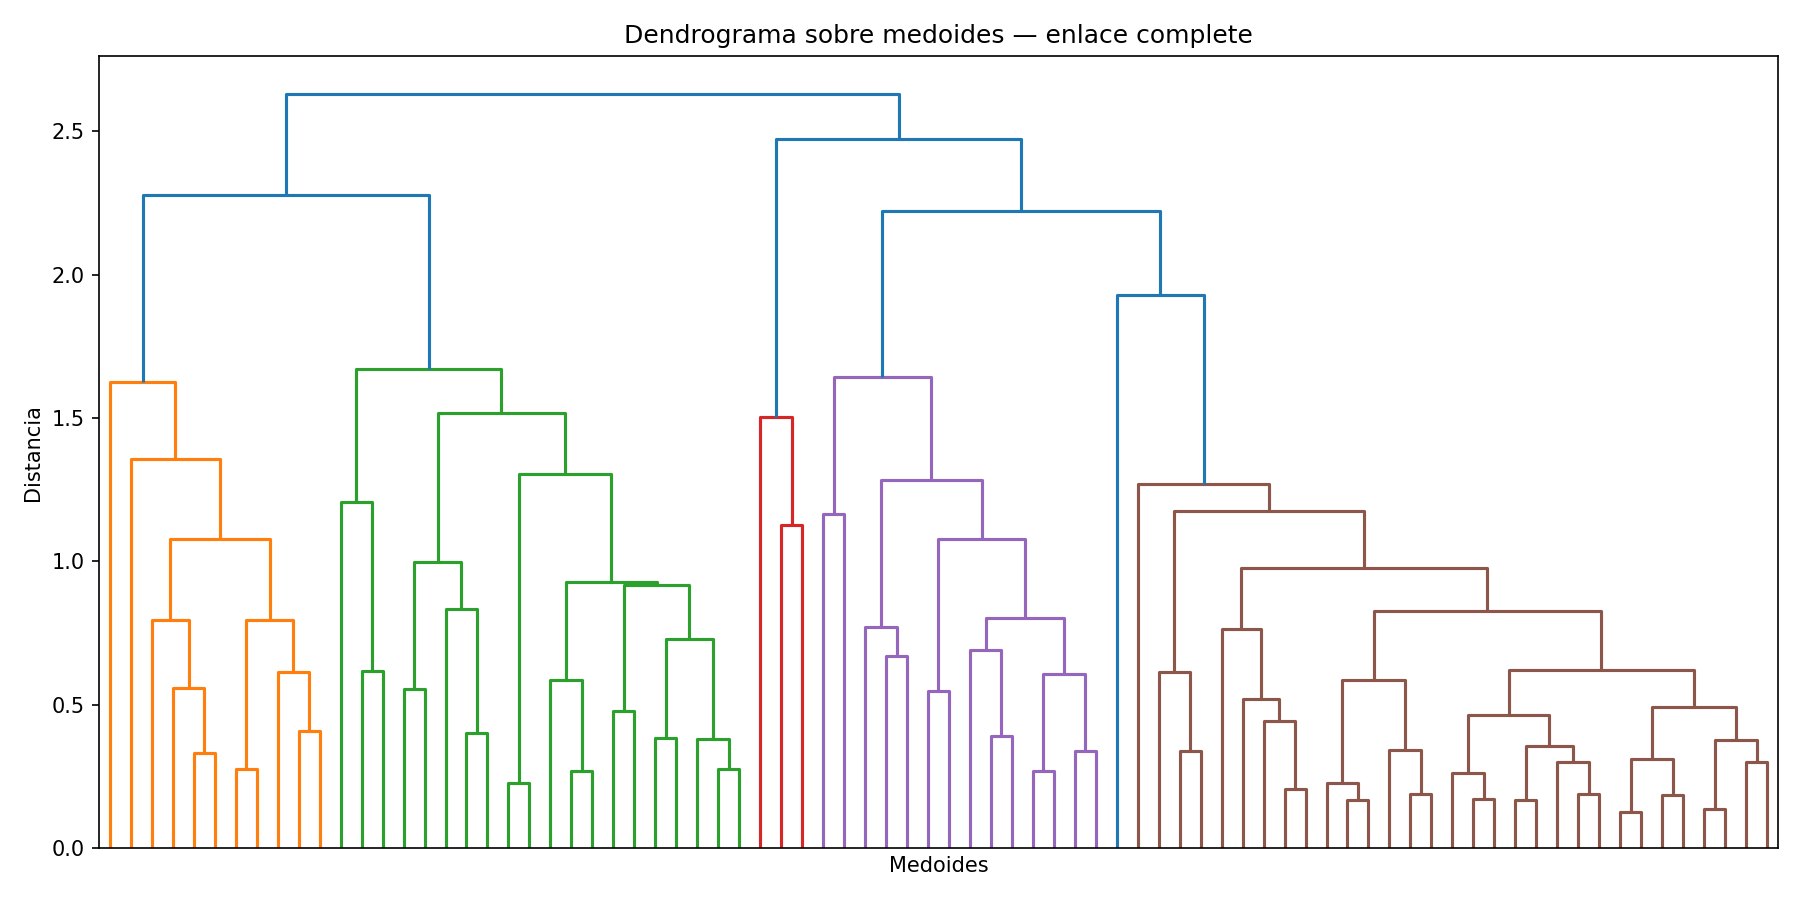
\includegraphics[width=\textwidth]{dendrograma_medoides_complete.png}
        \caption{Enlace completo}
        \label{fig:dendrograma_anuran_complete}
    \end{subfigure}
    \caption{Dendrogramas para Anuran Calls.}
    \label{fig:dendrogramas_anuran}
\end{figure}

Finalmente, se evaluaron diferentes valores de $k$ (número de grupos) en el rango de 2 a 12, calculando el \texttt{índice de Silhouette} para 
cada configuración (valor de $k$ y tipo de enlace). Los resultados se presentan en la \Cref{fig:silhouette_vs_k_hier_single_complete}.

\begin{figure}[H]
  \centering
  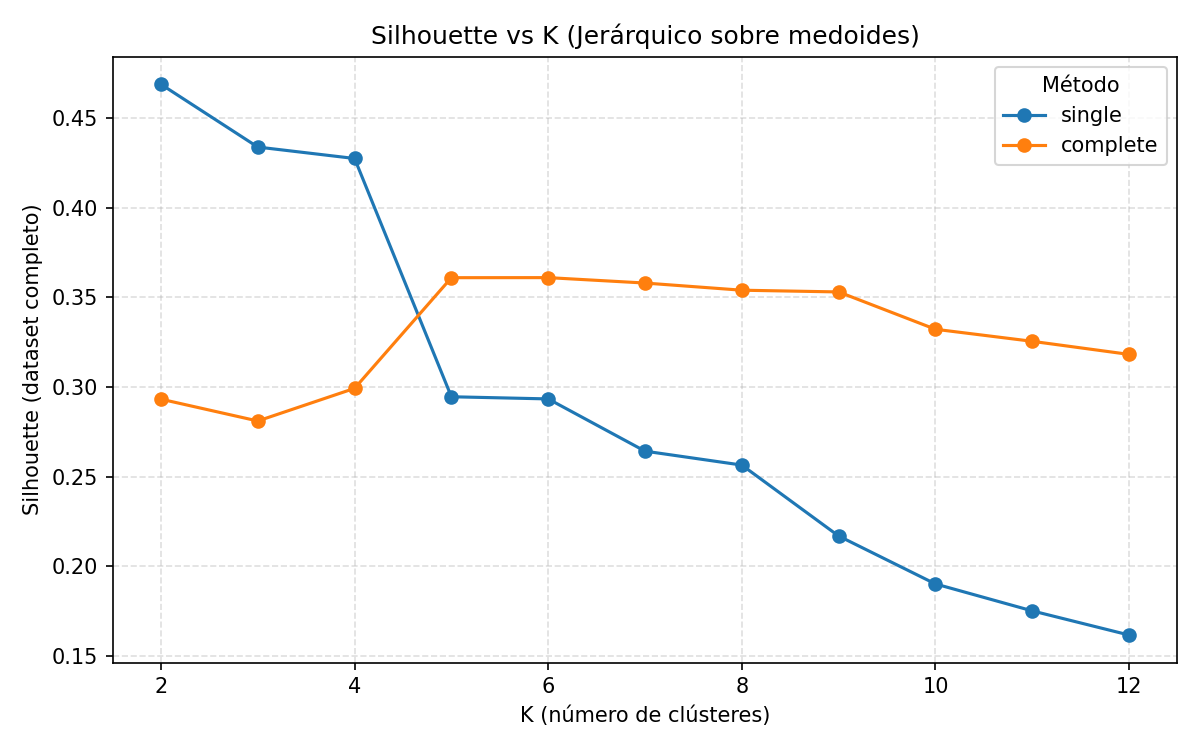
\includegraphics[width=\textwidth]{silhouette_vs_K_hier_single_complete.png}
  \caption{Silhouette para diferentes \(k\) y métodos de enlace.}
  \label{fig:silhouette_vs_k_hier_single_complete}
\end{figure}

Con base en los resultados obtenidos, se observa que el mejor rendimiento del índice de \textit{Silhouette} se alcanza con \(k=2\), 
utilizando el método de \emph{enlace completo}. Este hallazgo sugiere que, para el conjunto de datos \texttt{Anuran Calls},
la configuración óptima para el agrupamiento jerárquico es con dos grupos y empleando el criterio de enlace completo. No obstante, 
el coeficiente de \textit{Silhouette} obtenido es relativamente bajo, lo que indica que los grupos formados no están muy bien definidos y
que podría haber una considerable superposición entre ellos. Es posible que muchas de las características del conjunto de datos no sean 
relevantes para la tarea de agrupamiento, lo que dificulta la formación de grupos claros y distintos.

\subsubsection{Análisis Semi-supervisado}
Se fijó \(g=80\) protogrupos con K\textendash medoids (reusando lo definido en el ejercicio no supervisado). Sobre los medoides resultantes 
se construyó un agrupamiento jerárquico con dos tipos de enlace: \textit{single} y \textit{complete}. Para cada método se evaluaron cortes 
del dendrograma con \(K \in \{2,\dots,12\}\). Se generaron los dendrogramas y, para cada (método, \(K\)), se calculó el 
\texttt{índice de Silhouette} en el conjunto de entrenamiento ampliado (5\% etiquetado + 85\% no etiquetado), sin usar etiquetas. El mejor 
modelo jerárquico se determinó por el \texttt{índice de Silhouette}: entre todas las combinaciones (método, \(K\)) se eligió aquella con 
mayor \texttt{Silhouette}. Para hacer la tarea de clasificación, cada clúster final se rotuló con la etiqueta \texttt{Family|Genus} 
que resultó mayoritaria entre las observaciones del 5\% etiquetado que cayeron en ese clúster. Usando exclusivamente el 5\% etiquetado, se 
realizó validación cruzada para estimar el desempeño en clasificación del modelo seleccionado (método y \(K\) fijos por Silhouette). Los 
resultados de la métrica se presentan en la \Cref{fig:f1_score}.

\begin{figure}[H]
  \centering
  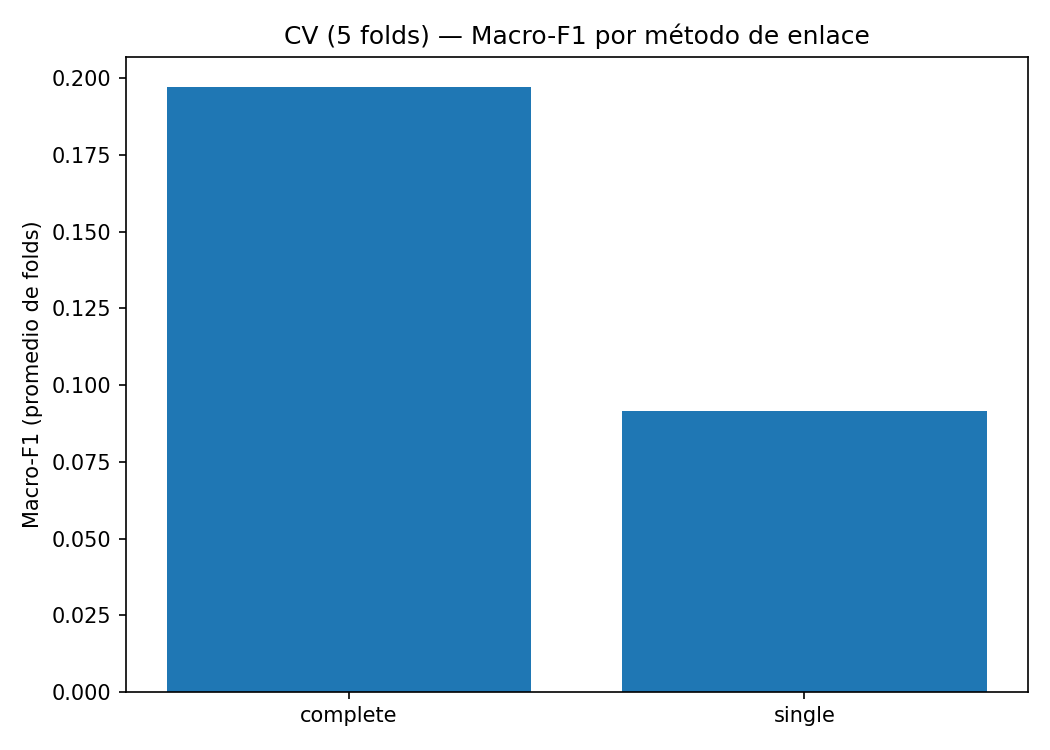
\includegraphics[width=0.7\textwidth]{cv_macroF1_por_metodo.png}
  \caption{F1 score para cada método de enlace.}
  \label{fig:f1_score}
\end{figure}

Dado que el mejor método de enlace fue \emph{complete linkage}, se construyó el modelo final replicando el procedimiento usado en la fase 
de selección, pero aplicado exclusivamente a este enlace. La \Cref{fig:dendograma_final} presenta el dendrograma resultante.

\begin{figure}[H]
  \centering
  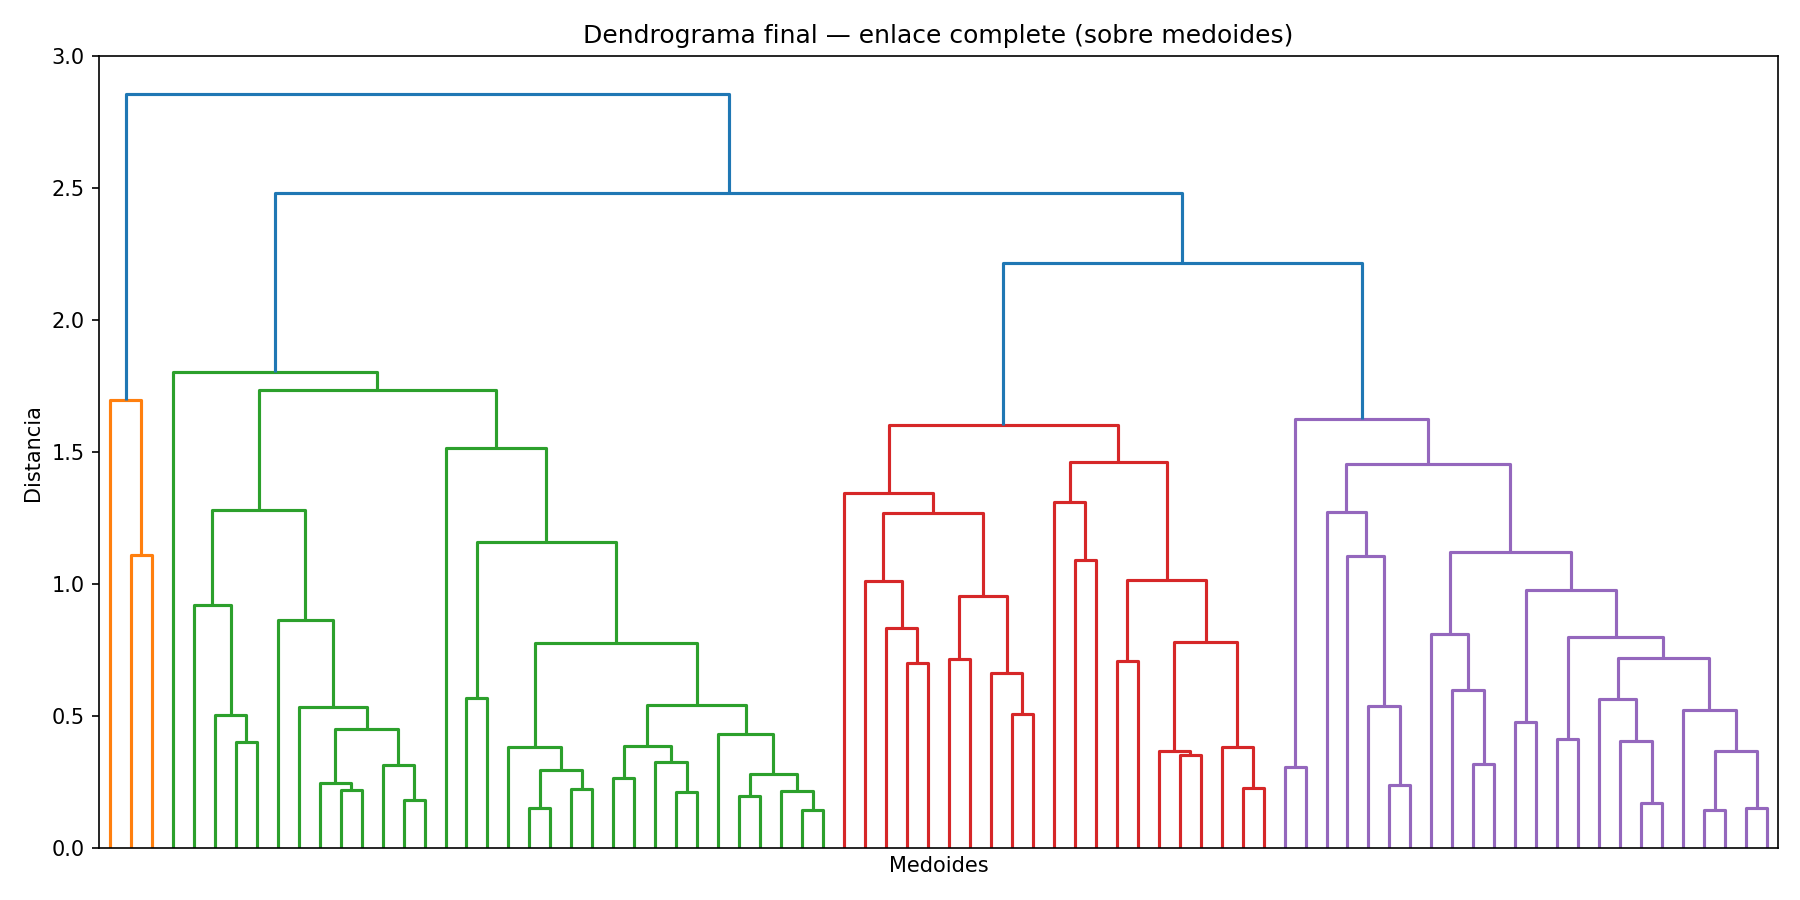
\includegraphics[width=\textwidth]{dendrograma_final_medoides_complete.png}
  \caption{Dendograma enlace completo enfoque semisupervisado.}
  \label{fig:dendograma_final}
\end{figure}

Con los clústeres definidos en el dendrograma y el valor óptimo del coeficiente de \textit{Silhouette} encontrado para \(k\) = 2. Las 
etiquetas se asignaron por mayoría utilizando el subconjunto etiquetado 5\%. Posteriormente, el modelo se evaluó en el conjunto 
de prueba (10\%), obteniéndose la matriz de confusión mostrada en la \Cref{fig:confusion_matrix_hierarchical_complete_k3}.

\begin{figure}[H]
  \centering
  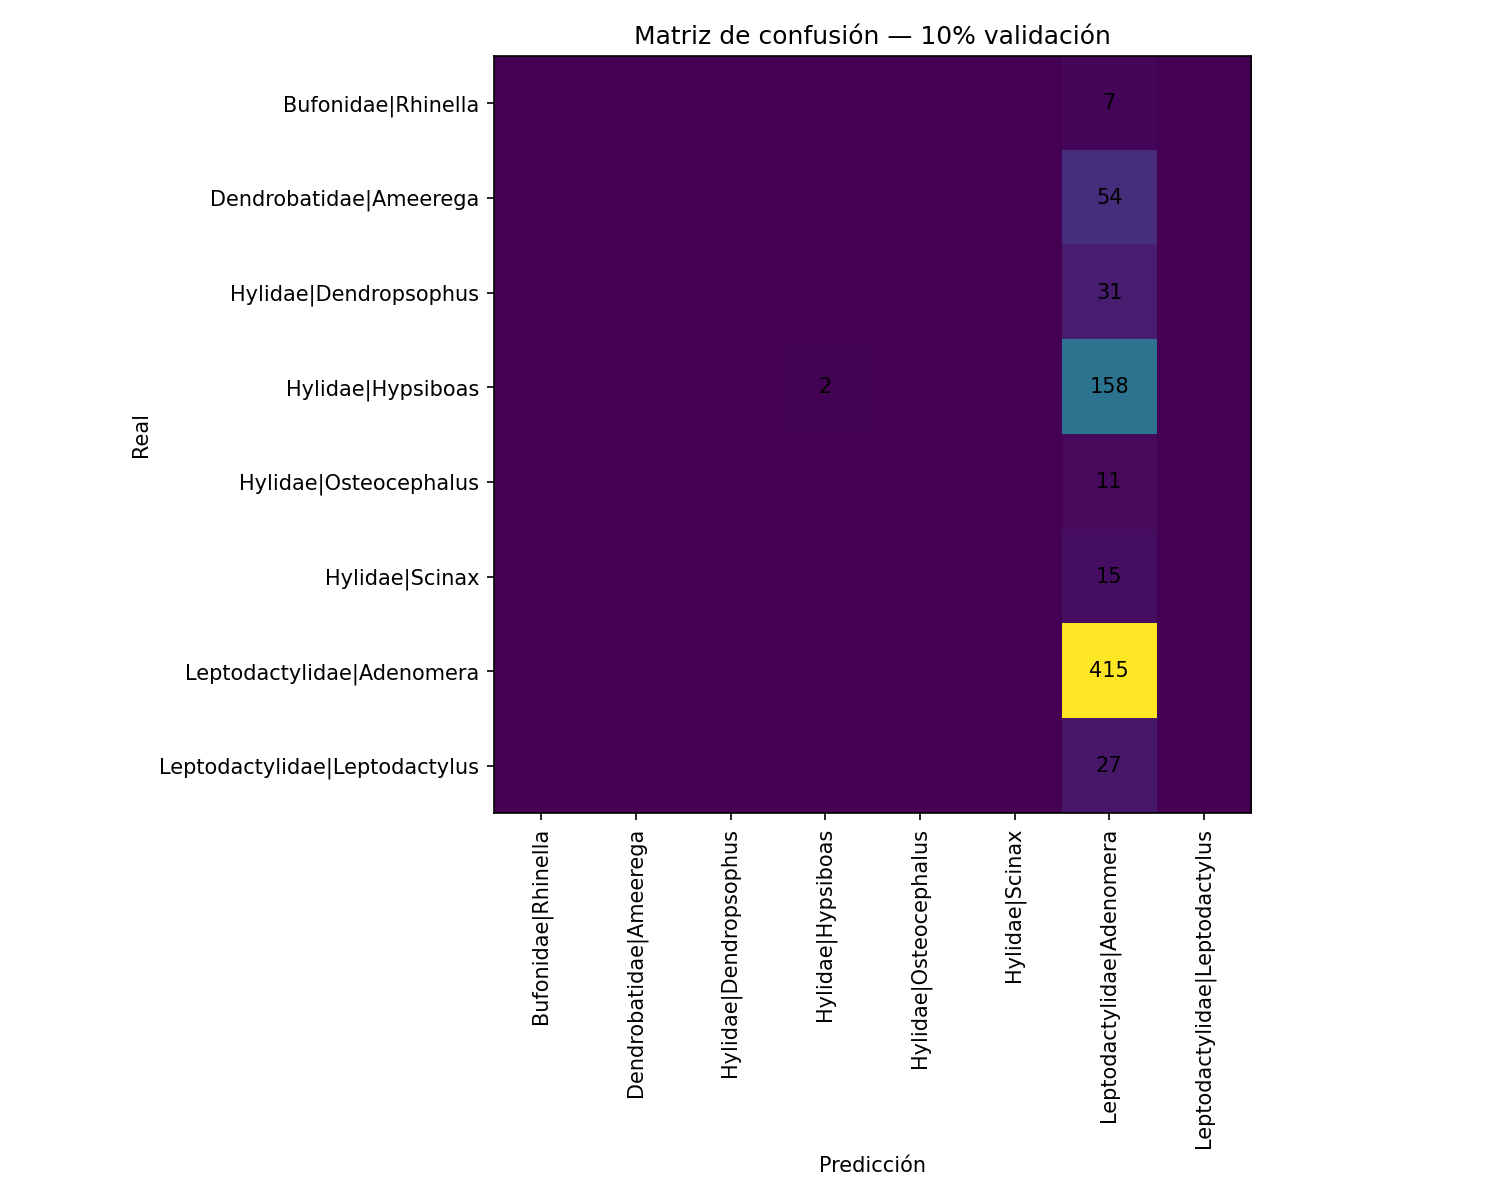
\includegraphics[width=0.7\textwidth]{matriz_confusion_validacion10.png}
  \caption{Matriz de confusión para \(k=2\) y enlace completo.}
  \label{fig:confusion_matrix_hierarchical_complete_k3}
\end{figure}

Con base en los resultados, el número óptimo de clústeres fue \(k\) = 2, por lo que el modelo jerárquico solo separa la muestra en dos
grupos y no logra representar las ocho clases reales del problema. Además, su desempeño es bajo (exactitud y precisión reducidas). 
Entre las posibles causas para este bajo desempeño se encuentran: 

\begin{itemize}
  \item Ausencia de un análisis de características que descarte colinealidad y variables ruidosas.
  \item Desbalance de clases. Es probable que la clase más frecuente esté sesgando la agrupación y la clasificación.
  \item Limitaciones del enfoque jerárquico para este dominio específico.
\end{itemize}

\section{Conclusiones}

\begin{itemize}
  \item En el caso del dataset \texttt{data\_clusters.mat}, los diferentes métodos de enlace produjeron resultados similares, sugiriendo que 
  el conjunto de datos tiene una estructura clara que puede ser capturada con varios enfoques.
  
  \item Para mejorar los resultados futuros, se recomienda realizar un análisis exhaustivo de las características para identificar y eliminar 
  variables redundantes o irrelevantes, así como considerar técnicas adicionales para manejar el desbalance de clases.

  \item No está del todo claro cómo definir el rango de búsqueda de \(k\) en el agrupamiento jerárquico ni en otras técnicas no supervisadas 
  vistas en clase. No existe un criterio estricto que justifique un rango específico; la literatura sugiere una relación entre el tamaño del 
  conjunto de datos y dicho rango, pero no constituye una norma, sino pautas heurísticas derivadas de la experimentación.

  \item La IA tiende a generar código generalista, a menudo no óptimo para casos específicos e, incluso, redundante o excesivo. Funciona mejor 
  cuando se le formulan \textit{prompts} breves y precisos, enmarcados en un contexto previo y claro del problema.

\end{itemize}

\end{document}
